% The original two-level training/calibration/prediction layout is preserved.
% Volume three architecture figures. Independent export only; not book fonts.
\colorlet{MutedBlueFill}{FigureBlueFill}
\colorlet{MutedGreenFill}{FigureGreenFill}
\colorlet{MutedPurple}{FigurePurple}
\colorlet{MutedPurpleFill}{FigurePurpleFill}
\tikzset{
 v3 picture/.style={x=1mm,y=1mm,font=\figurefont\fontsize{8}{10}\selectfont,text=FigureInk,line width=.65pt},
 v3 box/.style={draw=FigureBlue,fill=white,rounded corners=1.8pt,line width=.7pt,inner sep=2.5pt,align=center},
 v3 data/.style={v3 box,fill=FigureBlueFill},
 v3 model/.style={v3 box,draw=FigureGreen,fill=FigureGreenFill},
 v3 output/.style={v3 box,draw=FigureYellow,fill=FigureYellowFill},
 v3 risk/.style={v3 box,draw=FigureRed,fill=FigureRedFill},
 v3 group/.style={draw=FigureBlue,rounded corners=1.8pt,line width=.65pt,inner sep=3mm},
 v3 flow/.style={draw=FigureStroke,line width=.75pt,-{Stealth[length=1.65mm,width=1.05mm]},rounded corners=1pt},
 v3 guide/.style={draw=FigureMuted,line width=.6pt,dashed},
 v3 feedback/.style={v3 flow,draw=FigureGreen,dashed},
 v3 title/.style={draw=none,fill=none,font=\figurefont\fontsize{8}{10}\selectfont,align=center,inner sep=1pt},
 v3 note/.style={draw=none,fill=none,font=\FigureNoteFont\fontsize{7.5}{9.5}\selectfont,text=FigureMuted,align=center,inner sep=1pt},
 v3 label/.style={draw=none,fill=none,font=\figurefont\fontsize{8}{10}\selectfont,align=center,inner sep=1pt},
 v3 wire/.style={draw=FigureMuted,line width=.45pt},
 v3 point/.style={circle,draw=FigureBlue,fill=FigureBlueFill,minimum size=2.3mm,inner sep=0pt,line width=.55pt}
}
% Bring pre-existing native TikZ geometry to the same typography and scale.
\tikzset{
 foundation picture/.append style={font=\figurefont\fontsize{8}{10}\selectfont,line width=.65pt},
 foundation node/.append style={rounded corners=1.8pt,line width=.7pt,font=\figurefont\fontsize{8}{10}\selectfont},
 foundation heading/.append style={draw=none,fill=none,font=\figurefont\fontsize{8}{10}\selectfont},
 foundation note/.append style={draw=none,fill=none,font=\FigureNoteFont\fontsize{7.5}{9.5}\selectfont},
 foundation flow/.append style={line width=.75pt,-{Stealth[length=1.65mm,width=1.05mm]}},
 foundation frame/.append style={rounded corners=1.8pt,line width=.7pt},
 foundation edge label/.append style={draw=none,fill=none,font=\figurefont\fontsize{8}{10}\selectfont}
}
% Official Lucide outline icons, consistently used across diagrams. Size in mm.
\newcommand{\VIcon}[5]{\node[inner sep=0pt] at (#2,#3) {\includegraphics[width=#4mm]{figures/03-foundations/00-shared/tikz/icons/#1-#5.pdf}};}
% A neutral network glyph (not a claim about an actual model architecture).
% Coordinates denote its centre; scale 1 gives 13 x 8 mm.
\newcommand{\VNet}[4]{\begin{scope}[shift={(#1,#2)},scale=#3]
 \foreach \a in {-3,0,3}{\foreach \b in {-3,0,3}{\draw[v3 wire] (-5,\a)--(0,\b);}}
 \foreach \a in {-3,0,3}{\draw[v3 wire] (0,\a)--(5,0);}
 \foreach \a in {-3,0,3}{\draw[draw=#4,fill=#4,line width=.55pt] (-5,\a) circle(.9);\draw[draw=#4,fill=white,line width=.55pt] (0,\a) circle(.9);}
 \draw[draw=#4,fill=#4,line width=.55pt] (5,0) circle(.9);
\end{scope}}
\newcommand{\VDots}[4]{\foreach \k in {0,1,2,3}{\fill[#4] ({#1+2.7*\k},#2) circle(#3);}}
% Feature vector/tensor elements are scientific glyphs, not decorative icons.
\newcommand{\VVector}[4]{\foreach \k in {0,...,4}{\fill[#4,rounded corners=.25pt] ({#1+2.2*\k},#2) rectangle ++(1.5,#3);}}

% Detailed native teaching glyphs, reconstructed from the original Volume 3 art.
% Shared by this figure family; no title band, annotation box, shadow or texture.
\newcommand{\TBrain}[3]{\begin{scope}[shift={(#1,#2)},scale=#3]
 \path[draw=FigurePurple,fill=FigurePurpleFill,line width=.85pt,rounded corners=.4mm]
 (0,6.6) .. controls(-1.6,8.6)and(-4.2,8.4)..(-4.7,6.4) .. controls(-7.2,6.3)and(-8.1,4.6)..(-7.3,2.8) .. controls(-9.1,1.4)and(-8.9,-1.2)..(-7.4,-2.2) .. controls(-8.2,-4.4)and(-6.5,-6.7)..(-4.8,-6.4) .. controls(-4.1,-8.5)and(-1.4,-8.3)..(0,-6.8)
 .. controls(1.4,-8.3)and(4.1,-8.5)..(4.8,-6.4) .. controls(6.5,-6.7)and(8.2,-4.4)..(7.4,-2.2) .. controls(8.9,-1.2)and(9.1,1.4)..(7.3,2.8) .. controls(8.1,4.6)and(7.2,6.3)..(4.7,6.4) .. controls(4.2,8.4)and(1.6,8.6)..cycle;
 \draw[draw=FigurePurple,line width=.75pt] (0,6.6)--(0,-6.8);
 \draw[draw=FigurePurple,line width=1pt,line cap=round,line join=round] (-3.1,4.6)--(-3.1,1.1)--(-1.6,.1)--(-1.6,-5.5) (-5,1.3)--(-3.1,.2)--(-3.1,-2.5)--(-5,-3.7) (3.3,4.3)--(3.3,2.6)--(1.7,.7)--(1.7,-1) (5.4,1)--(3.7,-.5)--(3.7,-3.7)--(2.1,-5.1);
 \foreach \x/\y in {-3.1/4.6,-5/1.3,-5/-3.7,3.3/4.3,5.4/1,2.1/-5.1}{\draw[draw=FigurePurple,fill=white,line width=.8pt] (\x,\y) circle(.7);}
\end{scope}}
\newcommand{\TPerson}[5]{\begin{scope}[shift={(#1,#2)},scale=#3]
 \ifnum#5=1\def\pf{#4}\else\def\pf{white}\fi
 \draw[draw=#4,fill=\pf,line width=.65pt] (0,2) circle(1.55);
 \path[draw=#4,fill=\pf,line width=.65pt,rounded corners=.6pt] (-2.6,-3.5)--(-2.6,-1.4) arc[start angle=180,end angle=0,radius=2.6]--(2.6,-3.5)--cycle;
\end{scope}}
\newcommand{\TFolder}[5]{\begin{scope}[shift={(#1,#2)},scale=#3]
 \path[draw=FigureStroke,fill=#4Fill,line width=.75pt,rounded corners=.8mm] (-7,-4.5)--(-7,4.2)--(-3.5,4.2)--(-2,2.6)--(6,2.6)--(6,-4.5)--cycle;
 \ifnum#5=1\VEnvelope{0}{1.4}{.65}{FigureBlue}\fi
 \path[draw=FigureStroke,fill=#4Fill,line width=.75pt,rounded corners=.6mm] (-5.3,-4.5)--(-3.8,1)--(7,1)--(5.2,-4.5)--cycle;
\end{scope}}
\newcommand{\TBin}[5]{\begin{scope}[shift={(#1,#2)},scale=#3]
 \ifnum#5=1\begin{scope}[shift={(0,4)},rotate=-20]\VEnvelope{0}{0}{.7}{FigureBlue}\end{scope}\fi
 \path[draw=#4,fill=#4Fill,line width=.85pt,rounded corners=.7mm] (-4,3)--(-3.4,-6)--(3.4,-6)--(4,3)--cycle;
 \draw[draw=#4,line width=1.5pt,line cap=round] (-5,3)--(5,3);
 \draw[draw=#4,line width=.85pt,rounded corners=.5mm] (-1.8,3)--(-1.8,5)--(1.8,5)--(1.8,3);
 \foreach \x in {-2,0,2}{\draw[draw=#4,line width=.85pt,line cap=round] (\x,1)--(\x,-4.5);}
\end{scope}}
\newcommand{\TShield}[5]{\begin{scope}[shift={(#1,#2)},scale=#3]
 \path[draw=#4,fill=#4,line width=.65pt] (0,5.5) .. controls(1.9,4.2)and(3.6,3.8)..(4.4,3.5)--(4.4,-.4) .. controls(4.4,-3)and(2.2,-4.4)..(0,-5.7) .. controls(-2.2,-4.4)and(-4.4,-3)..(-4.4,-.4)--(-4.4,3.5) .. controls(-3.6,3.8)and(-1.9,4.2)..cycle;
 \ifnum#5=1\draw[draw=white,line width=1.2pt,line cap=round,line join=round] (-2.2,-.1)--(-.7,-1.8)--(2.6,1.7);\else\draw[draw=white,line width=1.2pt,line cap=round] (-1.7,-1.8)--(1.7,1.8) (-1.7,1.8)--(1.7,-1.8);\fi
\end{scope}}
\newcommand{\TTray}[4]{\begin{scope}[shift={(#1,#2)},scale=#3]
 \path[draw=#4,fill=#4Fill,line width=.85pt,rounded corners=.6mm] (-6,-3.3)--(-6,-.8)--(-3.8,3.3)--(3.8,3.3)--(6,-.8)--(6,-3.3)--cycle;
 \path[fill=#4,draw=#4,line width=.6pt,rounded corners=.4mm] (-6,-.3)--(-2.6,-.3)--(-1.9,-1.8)--(1.9,-1.8)--(2.6,-.3)--(6,-.3)--(6,-3.3)--(-6,-3.3)--cycle;
\end{scope}}
\newcommand{\TGear}[4]{\begin{scope}[shift={(#1,#2)},scale=#3]
 \foreach \a in {0,45,...,315}{\begin{scope}[rotate=\a]\path[draw=#4,fill=#4Fill,line width=.7pt,rounded corners=.4mm] (-1.5,3.3) rectangle (1.5,5.6);\end{scope}}
 \filldraw[draw=#4,fill=#4Fill,line width=.8pt] (0,0) circle(4.5);
 \filldraw[draw=#4,fill=white,line width=.8pt] (0,0) circle(2.1);
\end{scope}}
\newcommand{\TBalance}[3]{\begin{scope}[shift={(#1,#2)},scale=#3]
 \path[draw=FigureStroke,fill=FigureYellowFill,line width=.65pt,rounded corners=.35mm] (-1,-4.9)--(-.7,4.7)--(.7,4.7)--(1,-4.9)--(3,-5.5)--(3,-6)--(-3,-6)--(-3,-5.5)--cycle;
 \draw[draw=FigureYellow,line width=1.7pt,line cap=round] (-5.5,3.4)--(5.5,3.4);
 \filldraw[draw=FigureStroke,fill=FigureYellowFill,line width=.6pt] (0,4) circle(.8);
 \foreach \x in {-4,4}{\draw[draw=FigureStroke,line width=.6pt] (\x,3.4)--(\x-2.2,-1.2) (\x,3.4)--(\x+2.2,-1.2);\path[draw=FigureStroke,fill=FigureBlue,line width=.6pt] (\x-2.3,-1.2) arc[start angle=180,end angle=360,x radius=2.3,y radius=1.7]--cycle;}
\end{scope}}

\newcommand{\TOpenMail}[4]{\begin{scope}[shift={(#1,#2)},scale=#3,line join=round,line cap=round]
 \path[draw=FigureStroke,fill=#4Fill,line width=.75pt,rounded corners=.6mm] (-6,1)--(0,6.5)--(6,1)--(6,-5.2)--(-6,-5.2)--cycle;
 \draw[draw=FigureStroke,fill=white,line width=.7pt,rounded corners=.45mm] (-4.5,-1.5) rectangle (4.5,7.5);
 \foreach \y/\len in {5.5/5.5,3.5/5.5,1.5/4}{\draw[draw=#4,line width=.8pt] (-2.8,\y)--++(\len,0);}
 \path[draw=FigureStroke,fill=#4Fill,line width=.75pt,rounded corners=.6mm] (-6,1)--(0,-2.5)--(6,1)--(6,-5.2)--(-6,-5.2)--cycle;
 \draw[draw=FigureStroke,line width=.6pt] (-5.8,-5)--(-1.4,-1.7) (5.8,-5)--(1.4,-1.7);
\end{scope}}
% A uniform-tone variant preserves the reference neural glyph's layer count,
% filled circles and readable vertical spacing without replacing it by a logo.
\newcommand{\TNetwork}[7]{\begin{scope}[shift={(#1,#2)},scale=#3,yscale=1.15]
 \colorlet{VNetworkInput}{#7}\colorlet{VNetworkHidden}{#7}\colorlet{VNetworkOutput}{#7}
 \VLayerNet{0}{0}{1}{#4}{#5}{#6}
\end{scope}}

\begin{tikzpicture}[v3 picture]
\path[use as bounding box] (0,0) rectangle (163.2,98);
\node[v3 title] at (19,94) {独立训练样本};
\node[v3 data,minimum width=35mm,minimum height=23mm] (train) at (19,79) {};
\foreach \x/\y in {11/82,22/82,15/74,26/74}{\VDocument{\x}{\y}{0.7000}{FigureBlue}}
\node[v3 box,fill=FigureBlueFill,minimum width=24mm,minimum height=20mm] (fit) at (62,79) {};
\TNetwork{62}{79}{1.05}{2}{3}{1}{FigureBlue}
\node[v3 note] at (62,64) {固定 $f$ 与评分 $s$};
\draw[v3 flow] (train.east)--(fit.west);
\node[v3 title] at (105,94) {校准样本};
\node[v3 model,minimum width=31mm,minimum height=17mm] (cal) at (105,82) {};
\VDocument{98}{82}{0.7000}{FigureGreen}\VDocument{108}{82}{0.7000}{FigureGreen}
\node[v3 note] at (117,82) {$\cdots$};
\node[v3 box,draw=FigurePurple,fill=FigurePurpleFill,minimum width=27mm,minimum height=19mm] (score) at (105,56) {};
\TNetwork{105}{56}{1.05}{2}{3}{1}{FigureBlue}
\node[v3 note] at (82,51.5) {评分 $s$};
\draw[v3 flow] (cal.south)--(score.north);
\draw[v3 flow] (fit.east)--(84,79)--(84,61)--(score.west|-84,61);
\VIcon{lock-keyhole}{79}{79}{6}{ink}
\node[v3 title] at (148,94) {新预测输入 $x$};
\node[v3 data,minimum width=25mm,minimum height=17mm] (new) at (148,82) {};
\VDocument{148}{82}{0.8000}{FigureBlue}
\node[v3 box,draw=FigurePurple,fill=FigurePurpleFill,minimum width=27mm,minimum height=19mm] (predict) at (148,56) {};
\TNetwork{148}{56}{1.05}{2}{3}{1}{FigureBlue}
\draw[v3 flow] (new.south)--(predict.north);
% Frozen-model reuse is not calibration-score data flowing into prediction.
\draw[v3 guide] (score.east)--(predict.west);
\VIcon{lock-keyhole}{126.5}{56}{6}{ink}
\node[v3 note] at (126.5,62) {固定模型};
\draw[v3 flow] (score.south)--(105,37.5);
\node[v3 note] at (92,43) {校准分数};
\node[v3 box,minimum width=123mm,minimum height=37mm] (rank) at (62.5,19) {};
\node[v3 label] at (62.5,34) {$n=9,\quad\alpha=0.2$};
\node[inner sep=0pt] at (62.5,17) {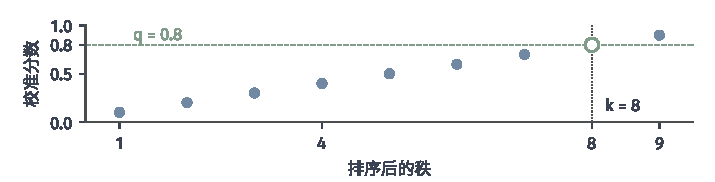
\includegraphics[width=121mm]{figures/03-foundations/03-trustworthiness/tikz/trust-conformal-construction/assets/panel.pdf}};
% The readable point prediction is inside the common circular core.
\VOperator{point}{148}{31}{14}{FigureBlue}{f(x)}
\draw[v3 flow] (predict.south)--(point.north);
\node[v3 label] at (137,22) {$C(x)$};
\node[v3 box,draw=FigureGreen,fill=FigureGreenFill,minimum width=30mm,minimum height=10mm] (interval) at (148,11) {};
\draw[v3 flow] (point.south)--(interval.north);
\draw[draw=FigureGreen,line width=1.4pt] (136,11)--(160,11);
\draw[draw=FigureGreen,line width=.9pt] (136,8.5)--(136,13.5) (160,8.5)--(160,13.5);
\filldraw[draw=FigureGreen,fill=FigureGreen!60!white] (148,11) circle(1.6mm);
\draw[v3 flow] (rank.east|-125,11)--(interval.west);
\node[v3 note] at (138,2) {$f(x)-q$};
\node[v3 note] at (158,2) {$f(x)+q$};
\end{tikzpicture}
